\section{Minimal number of measurements}

\todo[inline, color=yellow!40, bordercolor=yellow]{Prop 3.10 from Convex Geometry...}

\todo[inline, color=yellow!40, bordercolor=yellow]{Living on the Edge (definitions, theorem II, prop 4.5)}

\begin{figure}[t!]
    \centering
    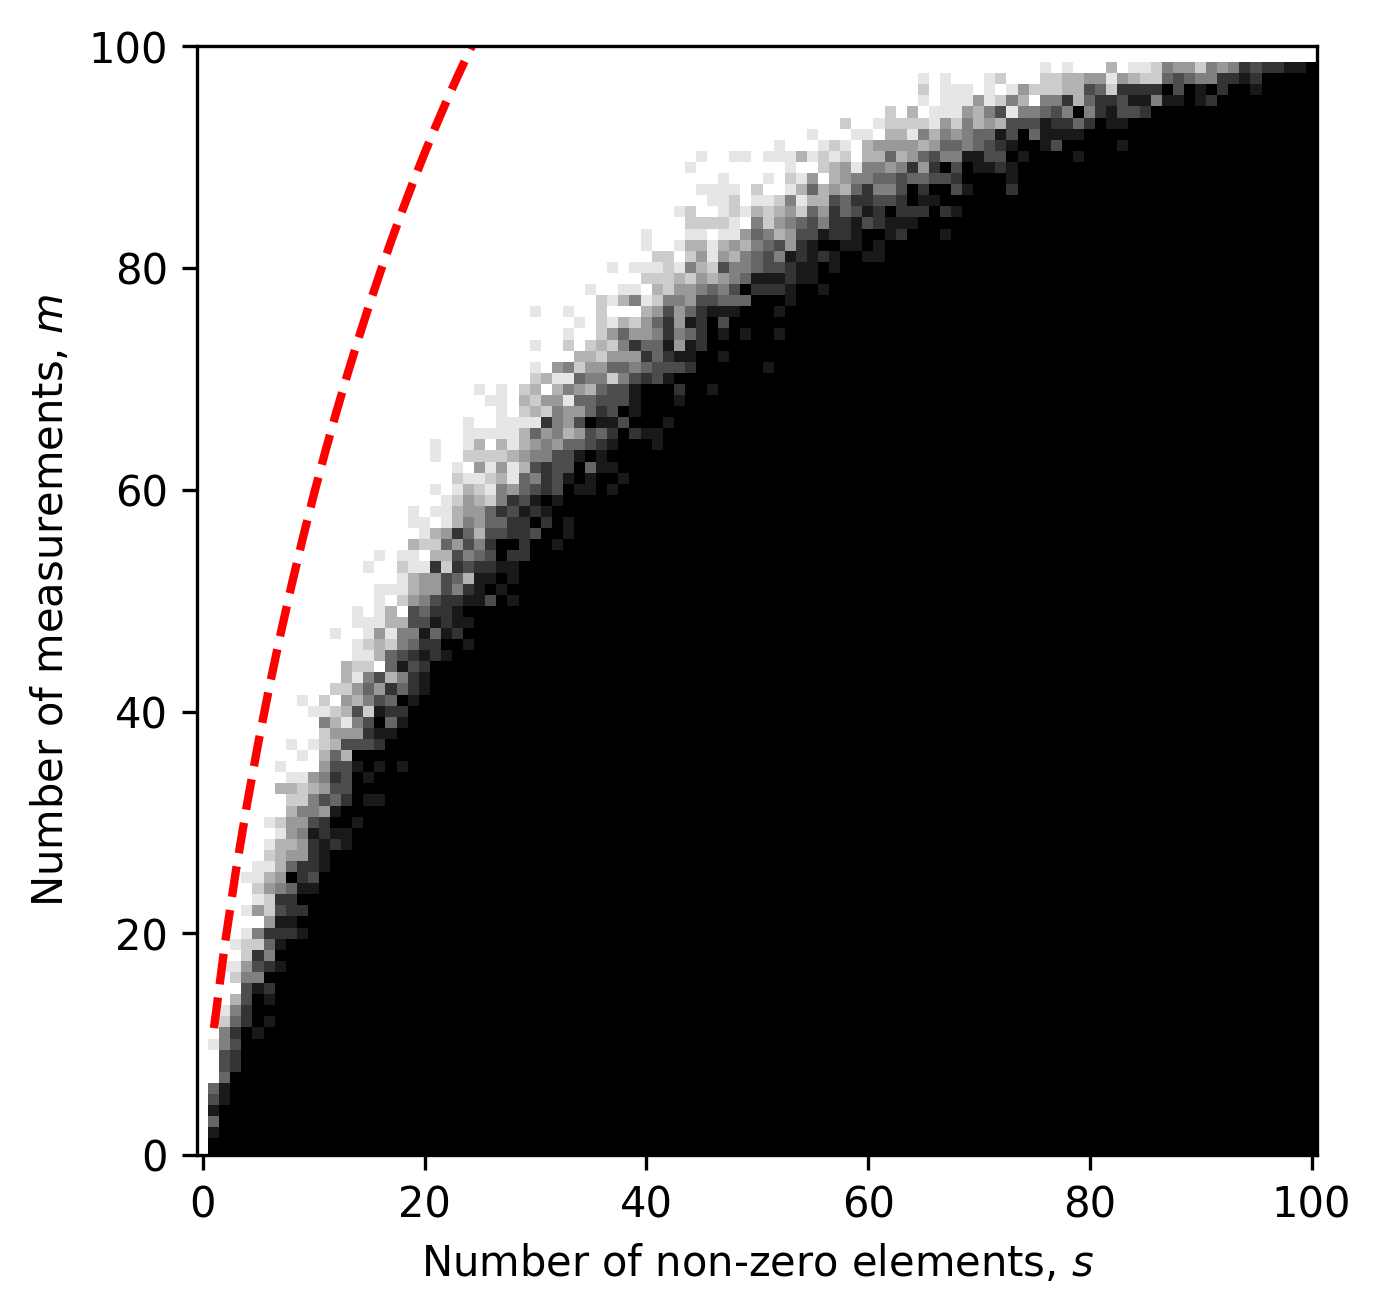
\includegraphics[width=0.5\textwidth]{pictures/log_estimate}
    \caption{Log}
    \label{fig:log}
\end{figure}

\begin{figure}
    \begin{subfigure}{0.5\textwidth}
            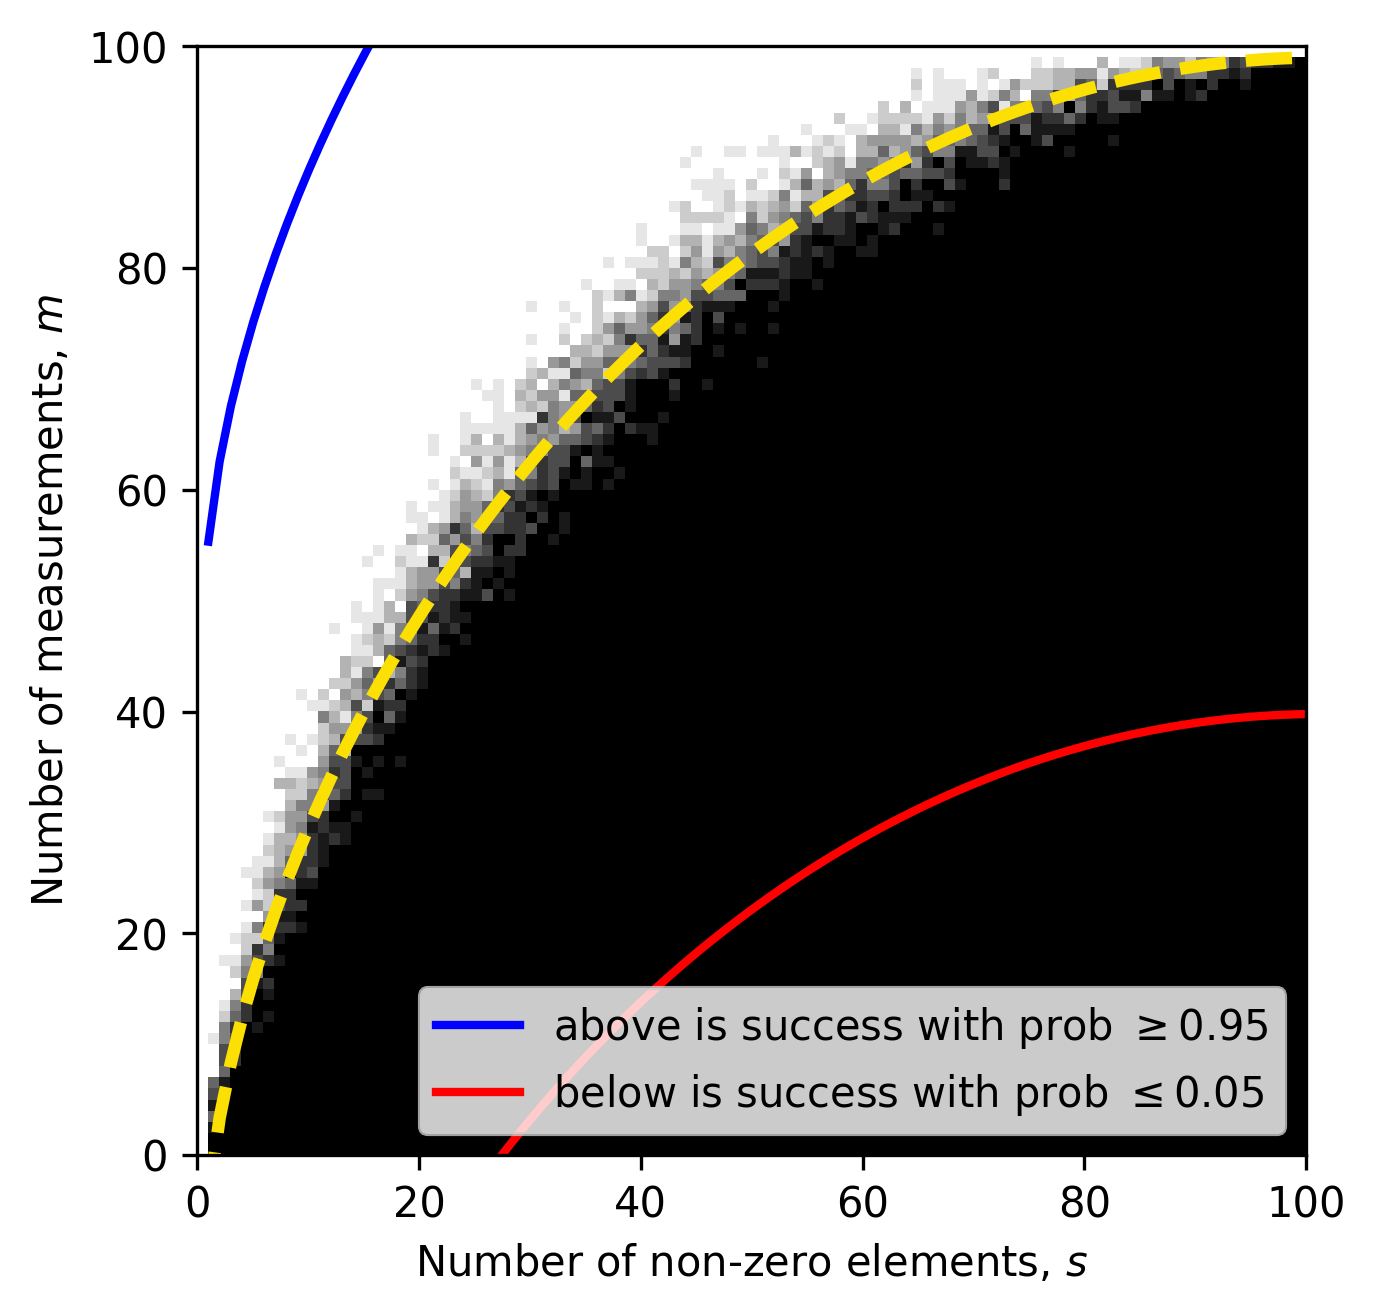
\includegraphics[width=\linewidth]{pictures/lote_estimates}
        \caption{}
    \end{subfigure}
    \begin{subfigure}{0.5\textwidth}
            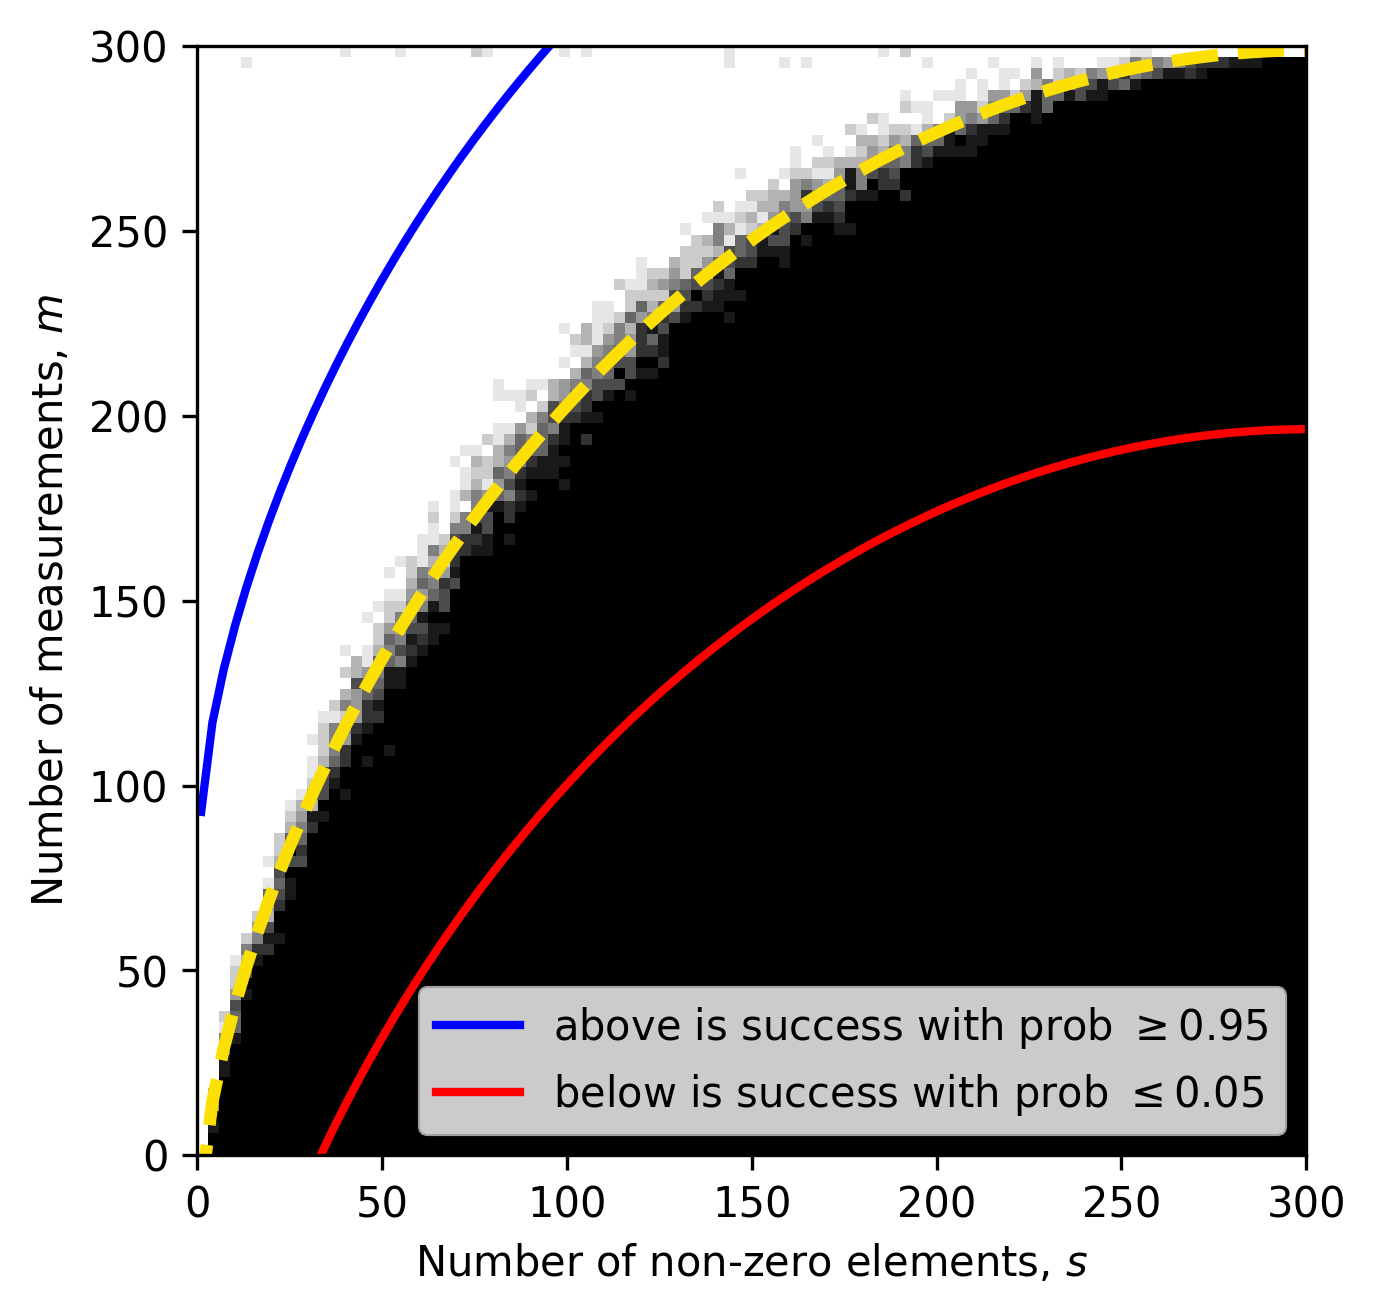
\includegraphics[width=\linewidth]{pictures/lote_estimates_d300}
        \caption{}
    \end{subfigure}

    \caption{Living on the Edge}
    \label{fig:lote}
\end{figure}


From now on we will consider only random matrices with $\mathcal{N}(0,1)$-distributed entries.
It might seem unnatural at first if we think of compressive sensing only in the context of natural phenomena.
However, another field of application is data compression; in that setting we are free to choose the matrix $\A$ however we like.
Considering the vast number of results for normally distributed matrices, they become the obvious candidates for study.

Before proceeding to recovery criteria for random matrices, we first have to recall some definitions from convex geometry.

\begin{definition}
    A convex set $\mathcal{C} \subset \mathbb{R}^N$ is called a \textit{cone} if it is closed under non-negative scalar multiplications, i.e.
    $\forall \alpha \geq 0, \x \in \mathcal{C}: \alpha \x \in \mathcal{C}$.

    The cone $\mathcal{C}^* = \{ \x \in \mathbb{R}^N : \left< \x, \y \right> \leq 0, \ \forall \y \in \mathcal{C} \}$
    is called the \textit{polar} of $\mathcal{C}$.
\end{definition}

\begin{definition}
    Let $C \subset \mathbb{R}^N$ be a convex set and $\x \in \mathbb{R}^N$.
    We call a \textit{tangent cone} of $C$ the cone $T_C(\x) = \op{cl}\{\alpha\x: \x \in C, \alpha > 0  \} $.
    We call a \textit{normal cone} of $C$ the cone $N_C(\x) = T_C^*(\x)$.
\end{definition}

\begin{definition}
    The \textit{descent cone} $\mathcal{D}(f, \x) $ of a proper convex function $f: \mathbb{R}^N \rightarrow \overline{\mathbb{R}}$
    at $\x \in \mathbb{R}^N$ is defined as $$\mathcal{D}(f, \x) = \bigcup_{\tau > 0} \left\{ \y \in \mathbb{R}^N: f(\x+\tau \y) \leq f(\x) \right\}. $$
\end{definition}

\begin{remark}
    Tangent cone to level sets
\end{remark}

\begin{proposition}
    The vector $\x$ is the unique solution of \ref{eq:l1} iff $\mathcal{D}(\norm{\cdot}_1, \x) \cap \op{Ker} \A = \{\mathbf{0}\}$.
\end{proposition}

\begin{proof}

\end{proof}

\begin{figure}
    \begin{subfigure}{0.45\textwidth}
        \begin{tikzpicture}
            \path [fill=teal, fill opacity=0.15] (0, 2) -- (-3.5, -1.5) to[curve through={(-2.5, -2.6) .. (-1.8, -2.7) .. (0, -3.4) ..
            (1.3, -2.9) .. (2, -2.8)}] (3.5, -1.5) -- (0, 2) --cycle;
            \draw [gray, densely dashed][->] (-3.5,0)--(3.5,0);
            \draw [gray, densely dashed][->] (0,-2.2)--(0,3);
            \draw [gray, densely dashed] (0, -3.5) -- (0, -2.8)
            \draw [teal, draw opacity=0.5] (0, 2) -- (-3.5, -1.5);
            \draw [teal, draw opacity=0.5] (0, 2) -- (3.5, -1.5);
            \draw [teal, line width=1pt][shorten <=-3cm] (0,2)--(3.5, 1) node [sloped, pos=0.7, above=-0.1cm] {$\op{Ker}\A+\x^*$};
            \draw [pattern=vertical lines, fill opacity=0.5](-2,0)--(0,2)--(2,0)--(0,-2)--cycle;
            \draw[black] [-{Circle[width=3pt, length=3pt, fill=black, black]}, shorten >=-1.5pt] (0,2) node [above right] {$\x^*$};
            \node at (0, -2.5) {$\mathcal{D}(\norm{\cdot}_1, \x^*)+\x^*$};
        \end{tikzpicture}
        \caption{}
    \end{subfigure}
    \hfill
    \begin{subfigure}{0.45\textwidth}
        \begin{tikzpicture}
            \path [fill=teal, fill opacity=0.15] (0, 2) -- (-3.5, -1.5) to[curve through={(-2.5, -2.6) .. (-1.8, -2.7) .. (0, -3.4) ..
            (1.3, -2.9) .. (2, -2.8)}] (3.5, -1.5) -- (0, 2) --cycle;
            \draw [gray, densely dashed][->] (-3.5,0)--(3.5,0);
            \draw [gray, densely dashed][->] (0,-2.2)--(0,3);
            \draw [gray, densely dashed] (0, -3.5) -- (0, -2.8)
            \draw [teal, draw opacity=0.5] (0, 2) -- (-3.5, -1.5);
            \draw [teal, draw opacity=0.5] (0, 2) -- (3.5, -1.5);
            \draw [teal, line width=1pt][shorten <=-1cm] (0,2)--(2.5, -3.5) node [pos=0, above left=0.3cm] {$\op{Ker}\A+\x^*$};
            \draw [fill=teal, fill opacity=0.15](-2,0)--(0,2)--(2,0)--(0,-2)--cycle;
            \draw[black] [-{Circle[width=3pt, length=3pt, fill=black, black]}, shorten >=-1.5pt] (0,2) node [above right] {$\x^*$};
            \node at (0, -2.5) {$\mathcal{D}(\norm{\cdot}_1, \x^*)+\x^*$};
        \end{tikzpicture}
        \caption{}
    \end{subfigure}
    \caption{descent cone}
\end{figure}

\todo[inline]{Here write about "Convex geometry of..."?}

\begin{definition}
    Atomic norm
\end{definition}

\begin{definition}
    Gaussian width
\end{definition}

\begin{proposition}
    Corollary 3.3(1)
\end{proposition}

\begin{proposition}
    Prop 3.10
\end{proposition}

\todo[inline]{Then about Living on the Edge}

\begin{definition}
    Intrinsic volume
\end{definition}

\begin{definition}
    Statistical dimension
\end{definition}

\begin{theorem}
    Theorem II
\end{theorem}


\begin{figure}
    \centering
    \includegraphics[width=0.8
    \textwidth]{pictures/compare_estimates}
    \caption{Comparison}
    \label{fig:compare}
\end{figure}